%%% COMPILE WITH XELATEX, NOT PDFLATEX
\documentclass[letterpaper]{article}
\author{L.M Goodman}
\date{September 2, 2014}
\title{Tezos --- a self-amending crypto-ledger \\ White paper}
%\usepackage[utf8]{inputenc}
%%\setlength{\parskip}{\baselineskip}
\usepackage{amsfonts}
\usepackage{listings}
\usepackage{color}
\usepackage{courier}
\usepackage{epigraph}
\usepackage{fontspec}
\usepackage{newunicodechar}
\usepackage{graphicx}
\usepackage{siunitx}
\usepackage{url}
\usepackage[hidelinks]{hyperref}



%\epigraphfontsize{\small\itshape}
\setlength\epigraphwidth{4.6cm}
\setlength\epigraphrule{0pt}
%\DeclareUnicodeCharacter{42793}{\tz{}}
%\newunicodechar{⚓}{\anchor}
%Ꜩ

\usepackage{url}
\lstset{basicstyle=\footnotesize\ttfamily,breaklines=true}

\newcommand{\tz}{{\fontspec{DejaVu Sans} \small{ꜩ}}}
\begin{document}

\maketitle

\epigraph{\emph{``Our argument is not flatly circular,
but something like it.''}}
{--- \textup{Willard van Orman Quine}}


\begin{abstract}
%% We present Tezos, a generic and self-amending crypto-ledger. Tezos can
%% instantiate any blockchain based ledger. The operations of a regular blockchain
%% are implemented as a purely functional module abstracted into a shell
%% responsible for network operations. Bitcoin, Ethereum, Cryptonote, etc. can all
%% be represented within Tezos by implementing the proper interface to the network
%% layer.
本白皮书向您介绍Tezos, 一个可以自我修正的加密数字账本。
Tezos的最大特点是可以容纳任何一种基于区块链的账本。 
在Tezos上,一个常规的区块链将仅仅被作为一个单纯的功能模块,通过负责网络运行的壳加以实现。
比特币,以太坊,Cryptonote等等都可以被在Tezos内实现通过实现对网络层面的接口。

%% Most importantly, Tezos supports meta upgrades: the protocols can evolve by
%% amending their own code. To achieve this, Tezos begins with a seed protocol
%% defining a procedure for stakeholders to approve amendments to the protocol,
%% \emph{including} amendments to the voting procedure itself. This is not unlike
%% philosopher Peter Suber's Nomic\cite{Nomic}, a game built around a fully
%% introspective set of rules.

更加重要的是,Tezos支持元升级,即协议可以通过修改自己的代码进行自我修正。
为实现这个目的,Tezos开始从一个种子协议来定义一整套流程来让持币的用户来对代码进行修正,甚至包括修正这套流程所必须的投票体系本身。这样一个建立在一整套内省规则之上的博弈和哲学家Peter Suber的Nomic博弈观点不谋而和。

%% In addition, Tezos's seed protocol is based on a pure proof-of-stake system
%% and supports Turing complete smart contracts. Tezos is implemented in OCaml,
%% a powerful functional programming language offering speed, an unambiguous
%% syntax and semantic, and an ecosystem making Tezos a good candidate for formal
%% proofs of correctness.
在此基础上,Tezos的种子协议被放在一个纯粹的PoS系统上,支持图灵完备的智能合约。Tezos通过OCaml 语言进行实现,该语言是一套功能强大的功能型编程语言,提供高速,含混度极低的词义和句法以及整个生态系统。所有的这一切让Tezos成为一个正式化证明系统的很好的候选人。

%% Familiarity with the Bitcoin protocol and basic cryptographic primitives are
%% assumed in the rest of this paper.
以下的白皮书要求读者要对比特币协议的一定程度的了解和并理解基本的加密学知识。

\end{abstract}
\newpage

\tableofcontents
\newpage

\section{简介}
%% In the first part of this paper, we will discuss the concept of abstract
%% blockchains and the implementation of a self-amending crypto-ledger.
%% In the second part, we will describe our proposed seed protocol.

在白皮书的第一部分,我们将讨论抽象区块链以及自动修复的加密账本的实现。在第二部分,我们将具体展开描述我们所倡导的种子协议。

\section{自动修复的加密数字账本}

一个区块链协议包含三层不同的协议:
\begin{itemize}
\item[-] 网络协议 ,发现并广播交易。
\item[-] -	交易协议,定义什么样的交易是合格的交易。
\item[-] -	共识协议,形成针对一个独特的链的共识。
\end{itemize}

%% Tezos implements a generic network shell. This shell is agnostic to the
%% transaction protocol and to the consensus protocol. We refer to the transaction
%% protocol and the consensus protocol together as a ``blockchain protocol''. We
%% will first give a mathematical representation of a blockchain protocol and then
%% describe some of the implementation choices
%% in Tezos.

Tezos配置了一个一般性的网络壳。这个壳是对交易协议和共识协议是完全独立和不干涉的。我们把转账协议和共识协议统称为区块链协议。我们将首先给一个区块链一个数学的表达,然后再对Tezos的各种功能的实现加以描述。

\subsection{数学表达}

%% A blockchain protocol is fundamentally a monadic implementation of concurrent
%% mutations of a global state. This is achieved by defining ``blocks'' as
%% operators acting on this global state. The free monoid of blocks acting on the
%% genesis state forms a tree structure. A global, canonical, state is defined as
%% the minimal leaf for a specified ordering.
一个区块链的协议本质上是一个不可再分的全局状态同步变化的monadic实现。这个实现的实现依赖于作为操作者(operator)的区块在该全球状态上提供的服务;这些不可再分状态的区块在创始状态之上形成一个树状结构。一个全球的被认可的状态就是这个树的满足一定顺序的最小叶。

%% This suggests the following abstract representation:
以下是其抽象的表达:

\begin{itemize}
\item[-] %% Let $(\mathbf{S},\leq)$ be a totally ordered, countable, set of possible
%% states.
让$(\mathbf{S},\leq)$定义为一个完全的类型化的,可以被计数的,可能状态的子集。
\item[-]%% Let $\oslash \notin \mathbf{S}$ represent a special, invalid, state.
把$\oslash \notin \mathbf{S}$代表一个特殊的无效的状态
\item[-]%% Let $\mathbf{B} \subset \mathbf{S}^{\mathbf{S} \cup \{\oslash\}}$ be the
%% set of blocks. The set of \emph{valid} blocks is
%% $\mathbf{B} \cap \mathbf{S}^{\mathbf{S}}$.
把$\mathbf{B} \subset \mathbf{S}^{\mathbf{S} \cup \{\oslash\}}$定义为区块。这个区块的集合是$\mathbf{B} \cap \mathbf{S}^{\mathbf{S}}$.
\end{itemize}

%% The total order on $\mathbf{S}$ is extended so that
%% $\forall s \in \mathbf{S}, \oslash < s$.
%% This order determines which leaf in the block tree is considered to be the
%% canonical one. Blocks in $\mathbf{B}$ are seen as operators acting on the state.
在$\mathbf{S}$之上的顺序被延续,所以这里$\forall s \in \mathbf{S}, \oslash < s$。而顺序决定了那个叶在区块树上是否被认可。区块在$\mathbf{B}$上被看做是在这个状态的操作者。

%% All in all, any blockchain protocol\footnote{GHOST is an approach which orders
%% the leafs based on properties of the tree. Such an approach is problematic for
%% both theoretical and practical reasons. It is almost always better to emulate it
%% by inserting proofs of mining in the main chain.} (be it Bitcoin, Litecoin,
%% Peercoin, Ethereum, Cryptonote, etc) can be fully determined by the tuple:
总而言之,任何一个区块链协议\footnote{GHOST是一种可以基于树特性对叶进行命令的方式。然而,这样的方式在理论和实践上都存在问题。与之相比,在主链添加挖矿证明几乎总是更好的解决方案。
所有这些区块链的网络协议在功能上大致相同,而基于参与者创造区块的动机的挖矿程序仅仅是一个新的网络特性。
},不论是比特币,莱特币,点点币,以太坊,还是Cryptonote,等等,都可以被完全用来被tuple来决定:
%% $$\left(\mathbf{S},\leq,\oslash,
%% \mathbf{B} \subset \mathbf{S}^{\mathbf{S} \cup \{\oslash\}}\right)$$
$$\left(\mathbf{S},\leq,\oslash,
\mathbf{B} \subset \mathbf{S}^{\mathbf{S} \cup \{\oslash\}}\right)$$

%% The networking protocol is fundamentally identical for these blockchains.
%% ``Mining'' algorithms are but an emergent property of the network,
%% given the incentives for block creation.
这些区块链的网络协议基本相同。其挖矿算法却发展迅速,激励着区块的创建。

%% In Tezos, we make a blockchain protocol introspective 
%% by letting blocks act on the protocol itself.
%% We can then express the set of protocols recursively as
%% $$\mathcal{P} = \left\{\left(\mathbf{S},\leq,\oslash,\mathbf{B} \subset
%% \mathbf{S}^{(\mathbf{S} \times \mathcal{P})\cup \{\oslash\}} \right)\right\}$$
Tezos使用区块链的协议,让区块在协议层面上运作。我们可以递归地表达这组协议:
$$\mathcal{P} = \left\{\left(\mathbf{S},\leq,\oslash,\mathbf{B} \subset
\mathbf{S}^{(\mathbf{S} \times \mathcal{P})\cup \{\oslash\}} \right)\right\}$$

\subsection{网络壳}
%% This formal mathematical description doesn't tell us \emph{how} to build the
%% block tree. This is the role of the network shell, which acts as an interface
%% between a gossip network and the protocol.
仅有一个形式的数学表述并不足以让我们立刻建立一个区块树。我们还需要一个连接Gossip网络和协议的网络壳。

%% The network shell works by maintaining the best chain known to the client. It is
%% aware of three type of objects. The first two are transactions and blocks, which
%% are only propagated through the network if deemed valid. The third are
%% protocols, OCaml modules used to amend the existing protocol. They will be
%% described in more details later on. For now we will focus on transaction and
%% blocks.
这个网络壳保证客户所认为的最优链正常运作。它将从三种对象那里接受信息。前两个是转账和区块,它们在被确认之后才通过网络进行广播。第三个是各种协议,即用来改变现有协议的OCaml模组,对此我们稍后再进行细致描述。
现在我们先把注意力放在转账和区块上。

%% The most arduous part of the network shell is to protect nodes against
%% denial-of-service attacks.
网络壳最艰巨的部分是保护节点免于遭受DOS攻击。

\subsubsection{时钟}
%% Every block carries a timestamp visible to the network shell. Blocks that appear
%% to come from the future are buffered if their timestamps are within a few
%% minutes of the system time and rejected otherwise. The protocol design must
%% tolerate reasonable clock drifts in the clients and must assume that timestamps
%% can be falsified.
每一个时钟带有一个自己的时间戳,这个时间戳只对网络外壳可视。如果一个区块是当前的,并且其时间戳在系统时间的几分钟之内,则该区块会被接受,否则则会被拒绝。这个协议在设计时考虑了宽容客户端的时钟的不一致,而且必须要假设时间戳可能会被伪造。

\subsubsection{链选择算法}
%% The shell maintains a single chain rather than a full tree of blocks. This chain
%% is only overwritten if the client becomes aware of a strictly better chain.
这个外壳保持一条单链,而不是一个完整的区块树。这个链只有在客户端获悉更优链条的时候才会被覆盖。

%% Maintaining a tree would be more parsimonious in terms of network communications
%% but would be susceptible to denial-of-service attacks where an attacker produces
%% a large number of low-scoring but valid forks.
建立一个完整区块树会更加节省资源,但也会让网络更加容易被DDOS攻击,尤其是当一个攻击者产生大量的低等级有效分叉的时候。

%% Yet, it remains possible for a node to lie about the score of a given
%% chain, a lie that the client may only uncover after having processed a
%% potentially large number of blocks. However, such a node can be subsequently
%% ignored.
但是仍然存在这样一种可能,那就是一个节点谎报了链的等级;而对一个客户端而言,这个谎言只能在大量的区块被处理后才能被发现, 而随后这个节点将被忽略。

%% Fortunately, a protocol can have the property that low scoring chains exhibit a
%% low rate of block creation. Thus, the client would only consider a few blocks of
%% a ``weak'' fork before concluding that the announced score was a lie.
幸运的是,一个协议可以被设计成具有这样的特性,那就是链的等级越低,打包块的速度也更慢,这样,客户端可能只需要查看某条链的几个区块,就可以判断它是不是一条错误的低等链。

\subsubsection{网络层防御}
%% In addition, the shell is ``defensive''.
%% It attempts to connect to many peers across various IP ranges. It detects
%% disconnected peers and bans malicious nodes.
壳具有防御性。它的目的是联系更多的不同IP波段的peers,并通过识别掉线的peers来防止对节点的恶意攻击。

%% To protect against certain denial of service attacks, the protocol provides the
%% shell with context dependent bounds on the size of blocks and transactions.
为防御特定DOS攻击,协议提供壳,而其所处的语境则基于区块大小的限制和转账大小。
\subsection{功能表述}

\subsubsection{验证链}

%% We can efficiently capture almost all the genericity
%% of our abstract blockchain structure with the following OCaml types.
%% To begin with, a block header is defined as:
我们可以通过以下的OCaml类型类非常有效地保证几乎所有的抽象区块链结构的通用性。从定义区块头开始:
\lstset{
  language=[Objective]Caml
}
\begin{lstlisting}
type raw_block_header = {
  pred: Block_hash.t;
  header: Bytes.t;
  operations: Operation_hash.t list;
  timestamp: float;
}
\end{lstlisting}

%% We are purposefully not typing the header field more strongly so it can
%% represent arbitrary content. However, we do type the fields necessary for the
%% operation of the shell. These include the hash of the preceding block, a list of
%% operation hashes and a timestamp. In practice, the operations included in a
%% block are transmitted along with the blocks at the network level. Operations
%% themselves are represented as arbitrary blobs.
我们故意没有把区块头类型化,这是为了更好地表述不同的内容。
然而我们一定要明确场的类型,以方便壳的正常运转。这些包括之前的区块的哈希,一系列运作的哈希值和一个时间戳。在实践中,一个区块内的运行被在区块一起在网络的层次上进行传播。
这些运行自己被代表为“arbitrary blobs”.


\begin{lstlisting}
type raw_operation = Bytes.t
\end{lstlisting}

%% The state is represented with the help of a \textbf{Context} module which
%% encapsulates a disk-based immutable key-value store. The structure of a
%% key-value store is versatile and allows us to efficiently represent a wide
%% variety of states.
在\textbf{Context}模块的帮助下,状态被表达,这包括了一个基于硬盘碟的不可修改的键值对的存储库。这个键值对的结构是非常灵活的,并且让我们可以非常有效地来代表很多种状态。

\begin{lstlisting}
module Context = sig
   type t
   type key = string list

   val get: t -> key -> Bytes.t option Lwt.t
   val set: t -> key -> Bytes.t -> t Lwt.t
   val del: t -> key -> t Lwt.t
   (*...*)
end
\end{lstlisting}

%% To avoid blocking on disk operations, the functions use the asynchronous monad
%% Lwt\cite{LWT}. Note that the operations on the context are purely functional:
%% \textbf{get} uses the \textbf{option} monad rather than throwing an exception
%% while \textbf{set} and \textbf{del} both return a new \textbf{Context}.
%% The \textbf{Context} module uses a combination of memory caching and disk
%% storage to efficiently provide the appearance of an immutable store.
为了避免阻塞存储碟的运行,这些功能使用非对称时序。注意,这个操作在语境上是纯功能性的:它使用通用的monad选项而不是搞例外地赋予这个返还值一个新的语境。这个语境模组使用内存和磁盘合并存储,目的是有效提供一个不可更改的存储环境。

%% We can now define the module type of an arbitrary blockchain protocol:
我们现在可以定义一个模组的类型,是一个含混的区块链协议:

\begin{lstlisting}
type score = Bytes.t list
module type PROTOCOL = sig
   type operation
   val parse_block_header : raw_block_header -> block_header option
   val parse_operation :  Bytes.t -> operation option

   val apply :
     Context.t ->
     block_header option ->
     (Operation_hash.t * operation) list ->
     Context.t option Lwt.t

   val score : Context.t -> score Lwt.t
   (*...*)
end
\end{lstlisting}

%% We no longer compare states directly as in the mathematical model, instead we
%% project the \textbf{Context} onto a list of bytes using the \textbf{score}
%% function. List of bytes are ordered first by length, then by
%% lexicographic order. This is a fairly generic structure, similar to the one used
%% in software versioning, which is quite versatile in representing various
%% orderings. 
和数学模型里不同,我们不需要去比较状态,而是通过得分功能把语境投射到一个字符列表。字符列一开始按长度排列,然后按照字母顺序排列 - 这个非常通用的结构和软件的版本排序类似,也在代表各种次序时被广泛应用。

%% Why not define a comparison function within the protocol modules? First off it
%% would be hard to enforce the requirement that such a function represent a
%% \emph{total} order. The score projection always verifies this (ties can be
%% broken based on the hash of the last block). Second, in principle we need 
%% the ability to compare states across distinct protocols. Specific protocol
%% amendment rules are likely to make this extremely unlikely to ever happen,
%% but the network shell does not know that.
为什么不在协议模块中定义比较的功能?
第一,	这样一个要求很难执行,也就是这样一个功能代表着一个完整的指令。评分的投放需要验证这些 - 根据上一个区块的哈希,连接有可能会被打断。
第二,	原则上我们需要可以对比不同平台状态的能力。具体的协议修改规则可能让这个发生的可能性变得非常低,但是网络的壳对此并不知情。

%% The operations \textbf{parse\_block\_header} and \textbf{parse\_operation} are
%% exposed to the  shell and allow it to pass fully typed operations and blocks to
%% the protocol but also to check whether these operations and blocks are
%% well-formed, before deciding to relay operations or to add blocks to the local
%% block tree database.
操作将区块头部和运行的设置被发送给网络壳,并允许操作和区块被传播,以及完整的操作被传达到区块协议上,但是在决定传递操作或者添加区块到本地树状数据库之前也会检查这些操作和区块是否是被很好地表达出来。

The apply function is the heart of the protocol:
申请功能将是协议的核心:

\begin{itemize}
\item[-]When it is passed a block header and the associated list of operations,
it computes the changes made to the context and returns a modified copy.
Internally, only the difference is stored, as in a versioning system,
using the block's hash as a version handle.
当它被传递到一个区块头部以及附属的操作时,它会运算对语境的改变并返还一个修改过的版本。在内部,只有改变被保存,就像在一个版本系统中一样,使用区块的哈希功能,作为版本的记号。
\item[-]When it is only passed a list of operations, it greedily attempts
to apply as many operations as possible. This function is not necessary for the
protocol itself but is of great use to miners attempting to form valid blocks.
当它只是被传递到一些操作的时候,它贪婪地试图申请尽可能多地申请操作。对于协议自身而言这些功能不是必须的,但对于矿工而言可以在形成有效区块时却是必须的。
\end{itemize}

\subsubsection{协议进化}

Tezos's most powerful feature is its ability to implement protocol capable
of self-amendment. This is achieved by exposing two procedures functions to the
protocol:
Tezos最强大的特性是它的协议自我修正能力。实现这一功能主要通过两套功能程序:

\begin{itemize}
\item[-] \textbf{set\_test\_protocol} which replaces the protocol
used in the testnet with a new protocol (typically one that has been adopted
through a stakeholder voter).
设立测试协议来替代测试网络中使用过的协议 (通常是一个被持币者投票所决定)
\item[-] \textbf{promote\_test\_protocol} which replaces the current
protocol with the protocol currently being tested
促进替代协议 - 用正在测试的协议替代目前正在运行的协议
\end{itemize}

These functions transform a Context by changing the associated protocol.
The new protocol takes effect when the following block is applied to the chain.
这些功能将通过改变目前的关联协议来转换语境。这些新的协议起效的时候也就是是一下的区块在链上生效的时候。

\begin{lstlisting}
module Context = sig
   type t
   (*...*)
   val set_test_protocol: t -> Protocol_hash.t Lwt.t
   val promote_test_protocol: t -> Protocol_hash.t -> t Lwt.t
end
\end{lstlisting}

The \textbf{protocol\_hash} is the \textbf{sha256} hash of a tarball of
\textbf{.ml} and \textbf{.mli} files. These files are compiled on the
fly. They have access to a small standard library but are sandboxed
and may not make any system call.
这个协议的哈希是tarball的.ml 和 .mli文件的sha256哈希。这些文件被在过程中集中起来。他们有基本的进入标准资源库的权限,但是被装在沙盒里,因此并不能对整个系统产生改变。

These functions are called through the \textbf{apply} function of the protocol
which returns the new \textbf{Context}.
这些功能被通过协议的应用功能产生作用,产生了新的语境。

Many conditions can trigger a change of protocol. In its simplest version,
a stakeholder vote triggers a change of protocol. More complicated rules
can be progressively voted in. For instance, if the stakeholder desire they
may pass an amendment that will require further amendments to provide a
computer checkable proof that the new amendment respects certain properties.
This is effectively and algorithmic check of ``constitutionality''.
很多的条件可能会触发协议修改条件。在最初的简单版本上,持币者可以通过直接投票进行协议修改, 而之后更复杂的协议可以通过逐步投票而获得接受。例如,当一个持币者希望一个修改案被通过,他会被要求提供计算机可以验证的证据来证明他的提案将会尊重协议的某些特性。这样,Tezos实现了有效的在程序上的宪法性。

\subsubsection{RPC}
In order to make the GUI building job's easier, the protocol exposes a JSON-RPC
API. The API itself is described by a json schema indicating the types of the
various procedures. Typically, functions such as \textbf{get\_balance} can
be implemented in the RPC.
为了实现GUI更容易地建立工作,这个协议暴露了JSONRPC的API.这个API自身可以被描述为一个代表各种程序类型的json schema。通常讲,很多功能都可以通过RPC来实现。

\begin{lstlisting}
type service = {
  name : string list ;
  input : json_schema option ;
  output : json_schema option ;
  implementation : Context.t -> json -> json option Lwt.t
}
\end{lstlisting}

The name is a list of string to allow namespaces in the procedures. Input and
output are optionally described by a json schema.
这个名字是一个列表的string,其目的是让名字的spaces出现在序列上。输入和输出是通过选择性json schema加以表述的。

Note that the call is made on a given context which is typically a recent ancestor
of the highest scoring leaf. For instance, querying the context six blocks above
the highest scoring leaf displays the state of the ledger with six confirmations.
注意这个指令被用来在一个特定的语境中,而这个语境经常是最高得分叶子的较近的祖先。例如,通过超过得分最高叶6个区块以上语境的询问,我们了解所有超过六个确认以上账簿的状态。

The UI itself can be tailored to a specific version of the protocol, or generically
derived from the JSON specification.
用户界面本身可以被根据加以修改来适应特定的协议版本,或者是由JSON的特定参数上推理得出。

\section{种子协议}
Much like blockchains start from a genesis hash, Tezos starts with a seed
protocol. This protocol can be amended to reflect virtually any blockchain based
algorithm.
就像区块链开始于一个初始哈希,Tezos开始于一个种子协议。这个协议可以被修改来反映几乎任何一个基于区块链的程序。

\subsection{经济}

\subsubsection{币量}
There are initially $\num{10000000000}$ (ten billion) coins, divisible up to two
decimal places. We suggest that a single coin be referred to as a ``tez''
and that the smallest unit simply as a cent. We also suggest to use the
symbol \tz~(\verb!\ua729!, ``Latin small letter tz'') to represent a tez.
Therefore 1 cent = \tz\num{0.01} = one hundreth of a tez.
Tezos一开始就会有一百亿个币,这些币小数点后保留两位。一个币被称作tez,而最小的单位是分。我们也建议使用ꜩ这个拉丁字母来代表一个tez。这样的话,一分等于0.01tez等于百分之一tez。

\subsubsection{挖矿和签名奖励}

\paragraph{原则}
We conjecture that the security of any decentralised currency requires
to incentivize the participants with a pecuniary reward. As explained in the
position paper, relying on transaction costs alone suffers from a tragedy of the
commons. In Tezos, we rely on the combination of a bond and a reward.
我们认为任何一个去中心化的货币都有赖于给参与者提供物质激励。
正如在我们的定位白皮书中提到的,仅仅依赖于转账费进行激励会导致公地悲剧。
在Tezos上,我们提供一个债券和现金奖励的二元激励体系。

Bonds are one year security deposits purchased by miners.
In the event of a double signing, these bonds are forfeited.
债券是一个矿工所购买的一年期的存款。当出现双重签名的情况下,这些债券将会被收回。

After a year, the miners  receive a reward along with their bond to compensate
for their opportunity cost. The security is primarily being provided by the
value of the bond and the reward need only be a small percentage of that value.
一年以后,矿工除了债券以外还将获得另外的奖励,作为他们机会成本的补偿。
债券和奖励的价值是系统安全的最主要保证,而它们的价值将仅占全部价值的一小部分。

The purpose of the bonds is to diminish the amount of reward needed, and perhaps
to use the loss aversion effect to the network's advantage.
债券是一个矿工所购买的一年期的存款。当出现双重签名的情况下,这些债券将会被收回。

\paragraph{细则}
In the seed protocol, mining a block offers a reward of \tz\num{512} and
requires a bond of \tz\num{1536}. Signing a block offers a reward of
$32\Delta T^{-1}$ tez where $\Delta T$ is the time interval in minutes between
the block being signed and its predecessor. There are up to 16 signatures per block
and signing requires no bond.
根据种子协议,每挖一个块将获得512个Tezos币现金奖励以及1536个币的债券奖励。而每一个一个签名将获得一个32∆T−1个tez的奖励。这里∆T代表以分钟表达的块被签名之间的时间间隔。每个块最多有16个签名,而仅仅签名并不能获得债券。

Thus, assuming a mining rate of one block per minute, about 8\% of the initial
money mass should be held in the form of safety bonds after the first year.
这样,假设一个挖矿的速度是每分钟出一个块,那么有8%的最初货币供应量应该在第一年后被以安全债券的形式被持有。

The reward schedule implies at most a 5.4\% \emph{nominal} inflation
rate. \emph{Nominal} inflation is neutral, it neither enrishes nor
impoverishes anyone\footnote{In contrast, Bitcoin's mining inflation impoverishes
Bitcoin holders as a whole, and central banking enrishes the financial
sector at the expense of savers}.
我们的奖励的时间表被设定为5.4%的最高通货膨胀率。正常的通货膨胀应该是中性的,它不会让有的人变富,而让其他人变穷。\footnote{与之相比, 比特币的挖矿的通货膨胀让比特币的持有者整体变穷,而中央银行又让金融界变得有钱,而让储户变穷。}.

Note that the period of a year is determined from the block's timestamps, not
from the number of blocks. This is to remove uncertainty as to the length of
the commitment made by miners. 
请注意这里的一年是根据区块的时间戳而不是区块的数量推算出来的,这是为了抵消矿工挖矿算力变化导致的不确定性。

\paragraph{展望}
The proposed reward gives miners a 33\% return on their bond.
This return needs to be high in the early days as miners and signers commit
to hold a potentially volatile asset for an entire year.
这个奖励机制将给矿工33%的债券回报。这个回报在初期必须要足够高,因为矿工和签名者必须承受早期币价的剧烈波动。

However, as Tezos mature, this return could be gradually lowered to the
prevailing interest rate. A nominal rate of inflation below 1\% could safely be
achieved, though it's not clear there would be any point in doing so.
但是,随着Tezos的成熟,这个回报可以被逐渐降低到一个同期的主流利率水平,并长期维持低于1%的形式通胀率,尽管这样做的必要性还需要进一步论证。

\subsubsection{丢失的币}
In order to reduce uncertainty regarding the monetary mass, addresses
showing no activity for over a year (as determined by timestamps)
are destroyed along with the coins they contain.
为了减少货币基数变化所带来的不确定性,所有的没有任何动作的地址和地址上所包含的币都会被销毁 - 这里的时间也是时间戳时间。

\subsubsection{修改规则}
Amendments are adopted over election cycles lasting $N = 2^{17} = \num{131072}$
blocks each. Given the  a one minute block interval, this is about three
calendar months. The election cycle is itself divided in four quarters of
$2^{15} = \num{32768}$ blocks. This cycle is relatively short to encourage early
improvements, but it is expected that further amendments will increase the
length of the cycle. Adoption requires a certain quorum to be met. This quorum
starts at $Q = 80\%$ but dynamically adapts to reflect the average
participation. This is necessary if only to deal with lost coins.
 修改政策可以被应用于选择周期,每个周期的长度为N=217=131072. 因为区块间隔是一分钟,所以这个间隔是三个月的时间。这个选举的周期被分成四阶段,每个阶段包含215天即32 768个区块。
这个周期相对比较短,这主要是为了激励早期的协议的改善。随着未来的修改,这个周期最终将变长。
被采纳整合会要求一个特定的quorum值被达到。这个quorum开始于Q=80%但是是动态地自我修正来反映平均的参与。

\paragraph{第一阶段}
Protocol amendments are suggested by submitting the hash of a tarball of
\verb!.ml! and \verb!.mli! files representing a new protocol. Stakeholders may
approve of any number of these protocols. This is known as ``approval voting'',
a particularly robust voting procedure.
协议修改被建议通过提交一个代表新协议的.ml和.mli的tarball的哈希开始。持币人可能会批准其中的任何一种协议。这也就是批准投票,是一个鲁棒性很强的投票程序。

\paragraph{第二阶段}
The amendment receiving the most approval in the first quarter is now subject to
a vote. Stakeholders may cast a vote for, against or can choose to explicitely
abstain. Abstentions count towards the quorum.
在第一阶段获得最多批准的修改案基础上进行投票。投票人可以投票反对或者弃权。弃权在计算quorum时被纳入统计。

\paragraph{第三阶段} If the quorum is met (including explicit abstentions),
and the amendment received $80\%$ of yays, the amendment is approved and
replaces the test protocol. Otherwise, it is rejected.
Assuming the quorum reached was $q$, the minimum quorum $Q$ is updated as such:
$$Q \leftarrow 0.8 Q + 0.2 q.$$
如果quorum被达到(包括明确的弃权),而修改案达到了80%的yays, 那么修改案就会被批准,并替代测试协议。否则它将被否决。
假设quorum的值是q,最小的quorum Q被升级到:
Q ← 0.8Q + 0.2q.

The goal of this update is to avoid lost coins causing the voting procedure to
become stuck over time. The minimum quorum is an exponential moving average of
the quorum reached over each previous election.
这个升级的目标是为了避免因为丢失币的问题延缓投票过程,因此以之前选举过程的指数性运动的quorum的平均数作为当前阶段quorum的下限。

\paragraph{第四阶段} Assuming the amendment was approved, it will have
been running in the testnet since the beginning of the third quarter.
The stakeholders vote a second time to confirm they wish to promote the test
protocol to the main protocol. This also requires the quorum to be met and an
$80\%$ supermajority.
假定修改案被批准,它将在第三阶段开始的时候开始测试网络运行。
持币者将进行第二次投票来确认他们确实想要支持测试协议进入主要协议。这也要求quorum下限被达到,以及80%的绝大多数投票者支持。


We deliberately chose a conservative approach to amendments. However,
stakeholders are free to adopt amendments loosening or tightening this policy 
should they deem it beneficial
我们故意地选择了一个保守的方法来进行修改。但是投票热 可以自由地去选择自己认为对有利的修改提议,并来对这个修改案进行适度的放松或者收紧。

\subsection{股权证明机制}

\subsubsection{概览}

Our proof-of-stake mechanism is a mix of several ideas, including
Slasher\cite{Slasher}, chain-of-activity\cite{CoA}, and proof-of-burn.
The following is a brief overview of the algorithm, the components of which
are explained in more details below.
我们的POS机制集成了几个不同的观念,其中包括Slasher, 活动链,烧币证明。以下的是一个简短的对程序的概览。这些概念将在以下被详细地介绍。

Each block is mined by a random stakeholder (the miner) and includes
multiple signatures of the previous block provided by random 
stakeholders (the signers). Mining and signing both offer a small reward but
also require making a one year safety deposit to be
forfeited in the event of a double mining or double signing.
每个块随机由矿工挖出,包括了此前一个块的随机提取的持币者的多个签名。挖矿和签名都将获得一笔小奖励,但是也要求存一笔一年期的押金,如果期间出现双挖或者双签,那么这笔押金将被没收。

The protocol unfolds in cycles of \num{2048} blocks. At the beginning of each
cycle, a random seed is derived from numbers that block miners chose and committed
to in the penultimate cycle, and revealed in the last. Using this random seed,
a follow the coin strategy is used to allocate migning rights and signing rights
to a specific addresses for the next cycle. See figure \ref{fig:pos_figure}.
这个协议在2048号块开始被运行。在每个周期的开始,一个随机种子将被通过由矿工所决定的一个数字推断得出,并被发送到penultimate cycle,并最后被展现出来。
通过使用随机种子,一个“跟随这个币”的策略被使用。这将被用在分配下一个周期的挖矿权利以及签名权利对一个确切地址。

\begin{figure}[b!]
  \centering
  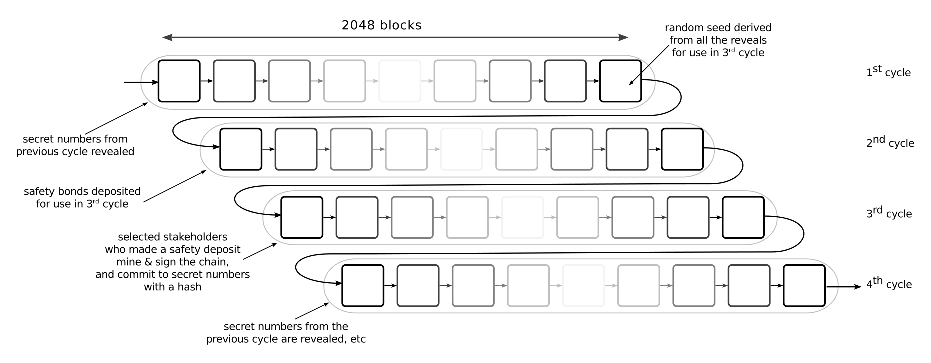
\includegraphics[width=0.8\textwidth]{pos_figure.eps}
  \caption{四周期POS机制}
  \label{fig:pos_figure}
\end{figure}


\subsubsection{时钟}

The protocol imposes minimum delays between blocks. In principle, each block
can be mined by any stakeholder. However, for a given block, each stakeholder
is subject to a random minimum delay. The stakeholder receiving the highest
priority may mine the block one minute after the previous block. The
stakeholder receiving the second highest priority may mine the block two
minutes after the previous block, the third, three minutes, and so on.
协议提供了最少的块之间的最小的延迟。原则上,任何一个持币人都可能挖出块。但是,就一个特定的块而言,每个持币者都将受到一个随机的最低延期的制约。最高优先级的持币人很可能会在上一个块出现后一分钟后挖出下一个。优先级第二的持币者可能在两分钟后挖到第二个个块,以此类推,优先级第三的会在三分钟后挖第三个块。

This guarantees that a fork where only a small fraction of stakeholder
contribute will exhibit a low rate of block creation. If this weren't 
the case, a CPU denial of service attacks would be possible by
tricking nodes into verifying a very long chain claimed to have a very high
score.
这套体系保证了弱分叉出块速度比主链要慢。否则,一个针对CPU的DDos攻击将可能欺骗节点以至于它会确认一个较长的自称高得分的链。

\subsubsection{随机种子生成}

Every block mined carries a hash commitment to a random number chosen by the
miner. These numbers must be revealed in the next cycle under penalty of
forfeiting the safety bond. This harsh penalty is meant to prevent selective
whitholding of the numbers which could be sued to attack the entropy of the seed. 
每一个被挖的块会贡献一个哈希值,被添加进矿工所决定的随机数。这些随机数必须在下一个周期的担保金没收时间前被公开。这个惩罚措施可以防止因矿工拒不提供随机数而有可能导致的对种子进行的熵攻击。

Malicious miners in the next cycle could attempt to censor such reveals, however
since multiple numbers may be revealed in a single block, they are very unlikely
to succeed.
恶意的矿工在第二步可能会试图阻止该随机数被公开,但是因为多个随机数会在单个区块中被公开,这样的企图很难成功。

All the revealed numbers in a cycle are combined in a hash list and the seed is
derived  from the root using the \verb!scrypt! key derivation function. The key
derivation should be tuned so that deriving the seed takes on the order of a
fraction of a percent of the average validation time for a block on a typical
desktop PC.
所有的被公开的数字在一个周期中都被合并在一个哈希列表中,而这个种子被从根部通过使用scrypt的密钥推断功能得出。这个密钥的推断必须要经过“调试”,因此推断种子所需的时间仅仅占一台普通桌面电脑确认区块所需时间的一小部分。

\subsubsection{Follow-the-coin过程}

In order to randomly select a stakeholder, we use a follow the coin procedure.
为了随机选取持币者,我们引入了一个跟随币机制。

\paragraph{原理}
The idea is known in bitcoin as follow-the-satoshi. The procedures works
``as-if'' every satoshi ever minted had a unique serial number. Satoshis are
implicitly ordered by creation time, a random satoshi is drawn and tracked
through the blockchain. Of course, individual cents are not tracked directly.
Instead, rules are applied to describe what happens when inputs are combined and
spent over multiple output.
这个方法最初出现在比特币中,成为“跟随中本聪”。
这个流程类似as-if指令。每一个聪单位的比特币都有一个独特的序列号,
而在比特币中,聪是被按照创始时间排序的,一个完全随机的聪被抽出,并且可以通过区块链进行追踪。
在Tezos系统里,单个分是不可以被追踪的。
但是可以通过使用一些规则将一些输入值集成起来,并通过多个输出花出。

In the end, the algorithm keeps track of a set of intervals associated with each
key. Each intervals represents a ``range'' of satoshis.
Unfortunately, over time, the database becomes more and more fragmented,
increasing bloat on the client side.
最后, 程序追踪每一组和密钥相联系的间隔。每一个间隔的作用等同于比特币中的聪。但这个办法的问题是,随着时间的延长,数据库变得越来越碎片化,客户端变得臃肿。

\paragraph{Coin Rolls}
We optimize the previous algorithm by constructing large ``coin rolls'' made up
of \num{10000} tez. There are thus about one million rolls in existence. A
database maps every roll to its current owner.
通过对之前代码的优化,我们采取了新的方法,即建立包含一万个tez组成的币卷。总共会有大约一百万个卷存在。一个数据库把每一个卷地图链接到它的目前的所有者那里。

Each address holds a certain set of specific rolls as well as some loose change.
When we desire to spend a fraction of a full roll, the roll is broken and
its serial number is sent in a LIFO queue of rolls, a sort of ``limbo''. Every
transaction is processed in a way that minimizes the number of broken rolls.
Whenever an address holds enough coins to form a roll, a serial number is pulled
from the queue and the roll is formed again.
每一个地址都带有一个特定组的特定卷,以及一些零钱。
当我们花掉只占一个卷一小部分的币时,整个卷就会被破坏,而它的序列号会在通过一个LIFO的卷的队列被发送出去。每一笔交易的处理过程中都尽量减少产生碎卷的数量。每当一个地址有足够的币来组成一个卷,一个序列号被从队列中提取,再次生成新卷。


The LIFO priority ensures that an attacker working on a secret fork cannot
change the coins he holds by shuffling change between accounts.
LIFO的优先级保证了攻击者无法通过在一个秘密分叉上挖矿然后通过洗账户的方法来修改其拥有的币数。

A slight drawback of this approach is that stake is rounded down to the
nearest integer number of rolls. However, this provides a massive improvement
in efficiency over the follow-the-satoshi approach.
这样做会有一个很小的问题,那就是“股份”数被近似取值为最接近的整数。但是相对于上述跟随中本聪方法,该方法在效率方面提供了很大的改善。

While the rolls are numbered, this approach does not preclude the use of 
fungibility preserving protocols like Zerocash. Such protocols can use
the same ``limbo'' queue technique.
尽管币卷被标了数字,这个方法并不能阻止那些诸如零币这样的比较注重互换性的协议被发明出来。这些协议可以使用相同的limbo序列技术。

\paragraph{动机}
This procedure is functionally different from merely drawing a random address
weighted by balance.
上述流程和仅仅抽取一个随机的按照余额分配比重选取地址的机制在功能上有很大的不同。

Indeed, in a secretive fork, a miner could attempt to control the generation of
the random seed and to assign itself signing and minting rights by creating the
appropriate addresses ahead of time. This is much harder to achieve if rolls
are randomly selected, as the secretive fork cannot fake ownership of certain
rolls and must thus try to preimage the hash function applied to the seed to
assign itself signing and minting rights. 
在一个秘密的分叉上,一个矿工可以试图通过控制随机种子的产生来提前来创造合适的地址以达到分配签名和挖币权的目的。然而如果币卷是真正随机被产生出来的,这种企图是非常难以成功的。这是因为秘密的分叉不能够伪造特定币卷的所有权归属,而且必须要试图来给哈希功能提前“造影” (preimage)来为自己分配签名和造币权。

Indeed, in a cycle of length $N=\num{2048}$, someone holding a fraction $f$ of
the rolls will receive on average $f N$ mining rights, and the effective
fraction received, $f_0$ will have a standard deviation of
$$\sqrt{\frac{1}{N}}\sqrt{\frac{1-f}{f}}.$$
事实上,在一个周期的长度N=2048的时候,某个占有f个币卷中一小部分的人将会获得平均值为fN的挖矿权,一旦这个有效的部分被收到,那么f0的标准偏差将为$$\sqrt{\frac{1}{N}}\sqrt{\frac{1-f}{f}}$$。

If an attacker can perform a brute-force search through $W$ different seeds,
then his expected advantage is at most\footnote{this is a standard bound
on the expectation of the maximum of W normally distributed variable}
$$\left(\sqrt{\frac{2\log(W)}{N}}\sqrt{\frac{1-f}{f}}\right)fN$$
blocks. For instance, an attacker controlling $f = 10\%$ of the rolls should
expect  to mine about $205$ blocks per cycle. In a secret fork where he attempts
to control the seed, assuming he computed over a trillion hashes, he could
assign itself about $302$ blocks, or about $14.7\%$ of the blocks. Note that:
如果一个攻击者可以进行对W进行穷举式搜索,那么他的攻击的优势最多是$$\left(\sqrt{\frac{2\log(W)}{N}}\sqrt{\frac{1-f}{f}}\right)fN$$个区块。
举个例子,如果一个攻击者控制了总量10%的币卷,那么他可以在每个周期挖205个块。假设他在试图控制种子的秘密分叉上运算了超过一万亿个哈希,那么他可以分配给自己占总量14.7%的302个块。注意:
\begin{itemize}
\item[-] The hash from which the seed is derived is an expensive key derivation
function, rendering brute-force search impractical.
产生种子的哈希是通过一个复杂的密钥推断功能产生的,这让穷举式攻击变得不现实。
\item[-] To make linear gains in blocks mined, the attacked needs to expend a
quadratically exponential effort.
要想通过挖块取得线性的收入增长,攻击者将需要动用指数型增长的资源。
\end{itemize}  


\subsubsection{挖矿}
The random seed is used to repeatedly select a roll. The first roll selected
allows its stakeholder to mine a block after one minute, the second one after
two minutes --- and so on. 
随机种子被不断用来选择币卷。第一个被选中的卷将给予它的拥有者一秒钟后挖块的权利,这个第二个可以在两分钟以后,以此类推。

When a stakeholder observes the seed and realizes he can mint a high priority
block in the next cycle, he can make a security deposit.
当一个持币者观察到种子并认识到他可以在下一个周期里挖掘一个高优先级的块的时候,他可以进行存币购买债券。

To avoid a potentially problematic situation were no stakeholder made a 
safety deposit to mine a particular block, after a 16 minutes delay, the
block may be mined without a deposit.
存在这样一个潜在问题,即没有人进行存币购买债券来挖一个特定的块。如果这种情况发生,那么在16分钟以后,这个块就可以在没有存币的情况下被挖出。

Bonds are implicitely returned to their buyers immediately in any chain
where they do not mine the block.
用于购买债券的币将在任何一个购币者没有在挖矿的链上被立刻返还。

\subsubsection{区块签名}
As it is, we almost have a working proof of stake system.
We could define a chain's weight to be the number of blocks.
However, this would open the door to a form of selfish mining.
就这样我们构建了一个几乎完备可行的股权系统。但是一个问题是定义一个链的重量为区块数量也带来了自私挖矿的问题。

We thus introduce a signing scheme. While a block is being minted, the random
seed is used to randomly assign 16 signing rights to 16 rolls. 
为此我们引入了一个签名机制。当一个区块被挖出的时候,随机产生的种子被随机地使用来分配16个签署权利给16个币卷。

The stakeholders who received signing rights observe the blocks being minted and
then submit signatures of that blocks. Those signatures are then included in
the next block, by miners attempting to secure their parent's inclusion in the
blockchain.
持币者获得签署权利后一旦观察到被挖出的区块就会上传区块签名。由于挖矿者试图里保证自己的母块被包含在区块链里,这些签名也因此被包括在下一个区块里。

The signing reward received by signers is inversely proportional to the time
interval between the block and its predecessor.
签名者获得的签名奖励和两个块之间的时间间隔成反比。

Signer thus have a strong incentive to sign what they genuinely believe to be
the best block produced at one point. They also have a strong incentive to agree
on which block they will sign as signing rewards are only paid if the block ends
up included in the blockchain.
签名者因此有很强的动机来尽快签署他们所认为的当前最优的块,也有很强的动机来就对哪个块签名达成共识,因为签名奖励只有在区块被合并进区块链后才能领取。

If the highest priority block isn't mined (perhaps because the miner isn't
on line), there could be an incentive for signers to wait for a while, just
in case the miner is late. However, other signers may then decide to sign the
best priority block, and a new block could include those signatures, leaving out
the holdouts. Thus, miners are unlikely to follow this strategy.
如果优先等级最高的块没有被挖出(可能是因为矿工没有在线)的时候签名者因为存在矿工迟到的可能性而决定等待。但是其它签名者可能会决定签署最高优先级的块,而一个新块可能包含这些签名,让那些等待者一无所获,所以矿工很可能不会采取等待的方法。

Conversely, we could imagine an equilibrium where signers panic and start
signing the first block they see, for fear that other signers will do so and
that a new block will be built immediately. This is however a very contrived
situation which benefits no one. There is no incentive for signers to think this
equilibrium is likely, let alone to modify the code of their program to act
this way. A malicious stakeholder attempting to disrupt the operations would only
hurt itself by attempting to follow this strategy, as others would be unlikely
to follow suit.
我们可以假设存在与之相反的情形,签名者过于担心竞争者抢先,而争相对所看到的第一个块进行签名。然而现实是这种情形其实对任何人没有什么好处。签名者不认为会出现这种状况,更不用说去修改他们的程序代码来去这样做。虽然理论上存在一个恶意的持币者试图扰乱秩序的可能,但这样只会损害自己的利益,其他人也不会效仿。

\subsubsection{链的权重}

The weight is the number of signatures.
链的重量被权重义为签名数。

\subsubsection{公开谴责机制}
In order to avoid the double minting of a block or the double signing of a
block, a miner may include in his block a denunciation.
为了避免双挖以及双签问题, 一个矿工或者可以在他的区块中加入一个公开谴责机制。

This denunciation takes the form of two signatures. Each minting signature
or block signature signs the height of the block, making the proof of malfeasance quite concise.
这个公开谴责机制的形式是双签名。每一个造币的签名或者块的签名都将显示块的高度,这让不良行为很难隐藏。

While we could allow anyone to denounce malfeasance, there is really no point to
allow anyone else beyond the block miner. Indeed, a miner can
simply copy any proof of malfeasance and pass it off as its own
discovery.\footnote{A zero-knowledge proof would allow anyone to benefit from
denouncing malfeasances, but it's not particularly clear this carries much
benefit.}
尽管我们可以允许任何人来谴责不良行为,但没有人比矿工更适合来这样做。
事实上,一个矿工可以简单地复制不良行为的证据并将其作为自己的发现而转达给其他人。

Once a party has been found guilty of double minting or double signing,
the safety bond is forfeited.
而一旦发现有双挖或者双签,那么安全保证金将被没收。

\subsection{智能合约}


\subsubsection{合约类型}
In lieu of unspent outputs, Tezos uses stateful accounts. When those
accounts specify executable code, they are known more generally as
contracts. Since an account is a type of contract (one with no
executable code), we refer to both as "contracts" in full generality.
和比特币的未被花输出不同,Tezos使用状态化账户。当这些账户规定了可被执行的代码时,它们也就成了广泛意义上的合约。

Each contract has a ``manager", which in the case of an account is 
simply the owner. If the contract is flagged as spendable, the manager
may spend the funds associated with the contract. In addition, each
contract may specify the hash of a public key used to sign or 
mine blocks in the proof-of-stake protocol. The private key may or
may not be controlled by the manager. 
每一个合约都有一个管理者,对于账户而言,这个管理者就是它的拥有者。如果这个合约被表明是可以被花的,那也意味着经理可以花这个合约相关联的资金。
另外,每一个合约都可能会规定一个公钥的哈希用来签署或者挖POS协议内的块。这个私钥既可以也可以不被管理人控制。

Formally, a contract is represented as:
正式的情况下,一个合同可以被代表为:

\begin{lstlisting}
type contract = {
  counter: int; (* counter to prevent repeat attacks *)
  manager: id; (* hash of the contract's manager public key *)
  balance: Int64.t; (* balance held *)
  signer: id option; (* id of the signer *)
  code: opcode list; (* contract code as a list of opcodes *)
  storage: data list; (* storage of the contract *)
  spendable: bool; (* may the money be spent by the manager? *)
  delegatable: bool; (* may the manager change the signing key? *)
}
\end{lstlisting}

The handle of a contract is the hash of its initial content. Attempting
to create a contract whose hash would collide with an existing contract
is an invalid operation and cannot be included in a valid block.
一个合同的handle是最初内容的哈希值。试图来创建一个合约,而这个合约的哈希值和已经存在的合同的哈希值相同是无效的,并且不能被整合进一个有效区块。

Note that data is represented as the union type.
请注意这个数据被呈现为一个union类型。

\begin{lstlisting}
type data =
  | STRING of string
  | INT of int
\end{lstlisting}

where \verb!INT! is a signed 64-bit integer and string is an array of
up to \num{1024} bytes. The storage capacity is limited to \num{16384} bytes,
counting the integers as eight bytes and the strings as their length.
当INT是一个被签名的64位integer,而string是一个1024字节的阵列,存储能力被限制在16384字节,并把integers作为一个八字节以及strings来作为它们的长度。

\subsubsection{起源}

The origination operation may be used to create a new contract, it specifies
the code of the contract and the initial content of the contract's storage. If
the handle is already the handle of an existing contract, the origination is
rejected (there is no reason for this to ever happen, unless by mistake or
malice).
起源操作可以被用来创造一个新的合约,它指定了一个合同的代码和初始的合同的内容。如果这个handle已经是一个已存合约的handle,那么起源将被拒绝(除非是因为错误或恶意,基本不会发生).

A contract needs a minimum balance of $\tz~\num{1}$ to remain active. If the
balance falls below this number, the contract is destroyed.
 一个合约需要一个最低的余额1来保证其正常运行。如果这个余额低于1,这个合约就会被销毁。
\subsubsection{交易}

A transaction is a message sent from one contract to another contract, this
messages is represented as:
一个交易是一个消息,被从一个合约发送到另外一个合约,这个消息被代表为:

\begin{lstlisting}
type transaction = {
  amount: amount; (* amount being sent *)
  parameters: data list; (* parameters passed to the script *)
  (* counter (invoice id) to avoid repeat attacks *)
  counter: int;
  destination: contract hash;
}
\end{lstlisting}

Such a transaction can be sent from a contract if signed using the manager's key
or can be sent programmatically by code executing in the contract. When the
transaction is received, the amount is added to the destination contract's
balance and the destination contract's code is executed. This code can make use
of the parameters passed to it, it can read and write the contract's storage,
change the signature key and post transactions to other contracts.
如果签名者通过管理人密钥签名,则可以通过一个合约发送交易,或者也可以以程序的方法通过合约内部的执行代码进行发送。
当这个交易被接受,这个交易金额就被加入指定合约的余额中,而该合约的代码就会被执行。这个代码将接受发送给它的参数,可以对合约的存储进行读和写的操作,改变签名密钥,以及转账信息发送给其它合约。

The role of the counter is to prevent replay attacks. A transaction is only
valid if the contract's counter is equal to the transaction's counter. Once a
transaction is applied, the counter increases by one, preventing the transaction
from being reused.
计数者起的作用是防止中继攻击。一个转账仅仅在合约的计数等于转账的计数的时候才有效。一旦一个转账被应用,这个计数者会增加1,防止转账被重新使用。

The transaction also includes the block hash of a recent block that the client
considers valid. If an attacker ever succeeds in forcing a long reorganization
with a fork, he will be unable to include such transactions, making the fork
obviously fake. This is a last line of defense, TAPOS is a great system to
prevent long reorganizations but not a very good system to prevent short term
double spending.
这个转账也可以包含一个客户端认为有效的且时间最近区块的哈希值。如果一个攻击者成功地迫使一个分叉进行长重组,这些个转账将不能被整合进区块链,这让这个分叉不被承认,这也是安全的最后一道防线。然而,虽然TAPOS是一个防止这种长重组非常有效,但是对于防止短期双花并不是十分有效。

The pair (account\_handle, counter) is roughly the equivalent of an unspent
output in Bitcoin.
这一对账户把手(account handle)和柜台(counter)的概念和比特币中一个没有被花掉的output差不多。

\subsubsection{存储费用}

Since storage imposes a cost on the network, a minimum fee of \tz~1 is assessed
for each byte increase in the storage. For instance, if after the execution of
a transaction, an integer has been added to the storage and ten characters have
been appended to an existing string in the storage, then \tz~18 will be withdrawn
from the contract's balance and destroyed. 
存储是网络上最重要的成本之一,一个最基本的费用是1字节增加在存储上所产生的费用。
例如,如果在一个转账被执行之后,一个integer被添加到存储中,而十个字节被添加到一个已经存在的存储的string上,然后\tz~18将被从合同的余额中被取出然后被销毁。


\subsubsection{代码}


The language is stack based, with high level data types and primitives and strict
static type checking. Its design is insipired by Forth, Scheme, ML and Cat.
A full specification of the instruction set is available in\cite{language}.
This specification gives the complete instruction set, type system and semantics
of the language. It is meant as a precise reference manual, not an easy introduction.
这个语言是基于占堆且具有静态的数据检测类型以及高等初始primitives。这个设计的灵感是Forth, Scheme, ML 和 Cat。它有一个完全描述的指令集,类型系统,以及词法和语义。一个精准的使用手册,而不是一个简单的介绍。

\subsubsection{费用}

So far, this system is similar to the way Ethereum handles transaction. However,
 we differ in the way we handle fees. Ethereum allows arbitrarily long programs
to execute by requiring a fee that increases linearly with the program's
executing time. Unfortunately, while this does provide an incentive for one
miner to verify the transaction, it does not provide such an incentive to other
miners, who must also verify this transaction. In practice, most of the
interesting programs that can be used for smart contracts are very short.
Thus, we simplify the construction by imposing a hard cap on the number of steps
we allow the programs to run for.
到目前为止,这个系统和以太坊处理转账的方式很类似。然而,我们在处理费用方面却很不同。在以太坊上用户只要交一个和处理长度线性对应的费用,就可以运行无限长的代码。
这样会有一个问题,就是它只给一个矿工验证这个转账提供经济动机,但并不能给同样必须参与这个转账的其他矿工相同的动机。在实践中,大多数可以被用来进行智能合约的有趣的程序是非常短的。这样我们通过加入一个硬性的上限来简化构建过程,并让我们的程序运行的最多步数。

If the hard cap proves too tight for some programs, they can break the execution
in multiple steps and use multiple transactions to execute fully. Since Tezos is
amendable, this cap can be changed in the future, or advanced primitives can be
introduced as new opcodes.
如果一个硬性的这个上限可能对一些程序过低,这些限制也可以通过使用多步运算的方式来进行提升,而使多个交易进行完全的运行。

If the account permits, the signature key may be changed by issuing a signed
message requesting the change.
基于Tezos可被修改的特性,这个上限具有未来被提升的空间,如果这个账户许可,这个签名的密钥可以被通过发送一个签名信息来进行修改。

\section{总结}
We feel we've built an appealing seed protocol. However, Tezos's true potential
lies in putting the stakeholders in charge of deciding on a protocol that they
feel best serves them.
我们认为我们已经建立了一个不错的种子协议。当然Tezos’ 的真正的潜力是让持币者有权利选择一个他们认为对自己最有利的协议。

\bibliographystyle{plain}
\bibliography{biblio}

\end{document}
